\documentclass[border=10pt]{standalone}
\usepackage{tikz}
\usepackage{amsmath}   % \overset 需要它
\usetikzlibrary{arrows.meta}
\definecolor{inFill}{RGB}{183,224,177}
\definecolor{inLine}{RGB}{32,102,32}
\definecolor{hidFill}{RGB}{199,203,243}
\definecolor{hidLine}{RGB}{52,58,143}
\definecolor{outFill}{RGB}{243,199,199}
\definecolor{outLine}{RGB}{143,52,52}
\definecolor{lineC}{RGB}{38,44,110}
\begin{document}
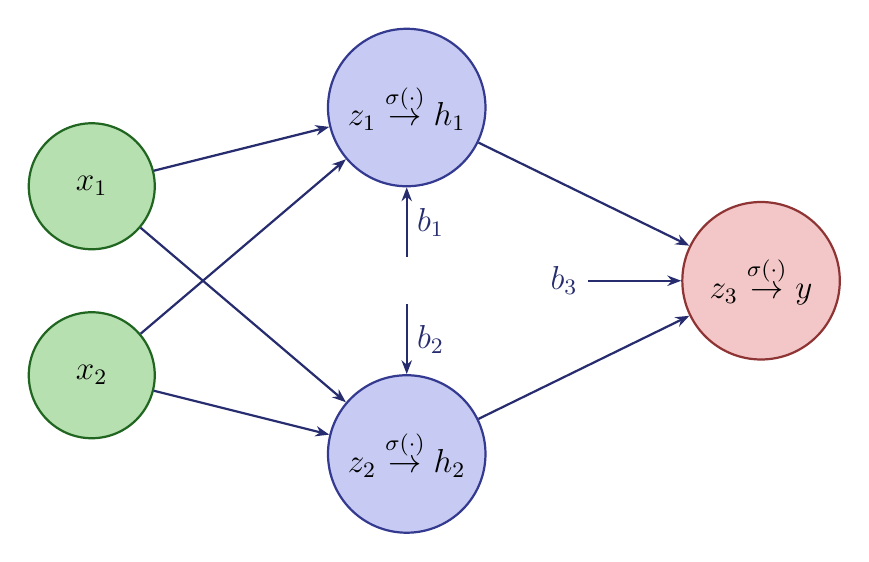
\begin{tikzpicture}[
    >={Stealth[length=5pt]}, line width=0.8pt, font=\large,
    inp/.style={circle, draw=inLine, fill=inFill, minimum size=1.6cm, inner sep=0pt},
    hid/.style={circle, draw=hidLine, fill=hidFill, minimum size=2.0cm, inner sep=1pt},
    outp/.style={circle, draw=outLine, fill=outFill, minimum size=2.0cm, inner sep=1pt},
    arr/.style={lineC, ->},
  ]
  % 节点：σ 叠在 ⇒ 上方
  \node[inp]  (x1) at (0, 1.2)  {$x_1$};
  \node[inp]  (x2) at (0,-1.2)  {$x_2$};
  \node[hid]  (h1) at (4, 2.2)  {$z_1 \overset{\sigma(\cdot)}{\rightarrow} h_1$};
  \node[hid]  (h2) at (4,-2.2)  {$z_2 \overset{\sigma(\cdot)}{\rightarrow} h_2$};
  \node[outp] (y)  at (8.5, 0)  {$z_3 \overset{\sigma(\cdot)}{\rightarrow} y$};

  % 全连接箭头
  \foreach \i in {x1,x2}
    \foreach \j in {h1,h2}
      \draw[arr] (\i) -- (\j);
  \draw[arr] (h1) -- (y);
  \draw[arr] (h2) -- (y);

  % 偏置箭头
  \draw[arr] (4, 0.3)  -- (h1) node[midway, right] {$b_1$};  % 正下方 → 竖直向上指 h1
  \draw[arr] (4,-0.3)  -- (h2) node[midway, right] {$b_2$};  % 正上方 → 竖直向下指 h2
  \draw[arr] (6.3, 0)   -- (y)  node[pos=0, left]  {$b_3$};
\end{tikzpicture}
\end{document}